%------------------------------------------------
\section{Multi-Level Feedback Queue}
%------------------------------------------------

\begin{frame}{Multi-Level Feedback Queue (MLFQ)}
    \begin{itemize}
        \item MLFQ addresses two main scheduling goals:
        \begin{itemize}
            \item Minimize \textbf{turnaround time}.
            \item Minimize \textbf{response time} for interactive jobs.
        \end{itemize}

        \item Challenge:
        \begin{itemize}
            \item The OS usually does not know how long a job will run.
            \item SJF/STCF require such knowledge.
            \item Round Robin improves responsiveness but may hurt turnaround time.
        \end{itemize}
    \end{itemize}

    \begin{block}{The Crux}
        How can a scheduler achieve good response and turnaround times
        without a priori knowledge of job length?
    \end{block}
\end{frame}

%------------------------------------------------

\begin{frame}{Learning From History}
    \begin{itemize}
        \item MLFQ uses the \textbf{observed behavior} of jobs to determine priorities.
        \item It uses past behavior to predict future behavior.
        \item Interactive jobs tend to:
        \begin{itemize}
            \item run for short periods;
            \item frequently relinquish the CPU for I/O.
        \end{itemize}
        \item CPU-bound jobs tend to use the CPU for long periods.
    \end{itemize}
\end{frame}

%------------------------------------------------

\begin{frame}{MLFQ: Basic Structure}
    \begin{columns}
        \column{0.55\textwidth}
        \begin{itemize}
            \item MLFQ contains multiple queues with different priority levels.
            \item A ready job belongs to exactly one queue.
            \item Higher-priority jobs run before lower-priority jobs.
            \item Jobs at the same priority are scheduled using Round Robin.
        \end{itemize}

        \begin{block}{Basic Rules}
            \textbf{Rule 1:} If Priority(A) $>$ Priority(B), A runs.\\[0.3em]
            \textbf{Rule 2:} If Priority(A) = Priority(B), A and B run in RR.
        \end{block}

        \column{0.45\textwidth}
        \begin{figure}
            \centering
            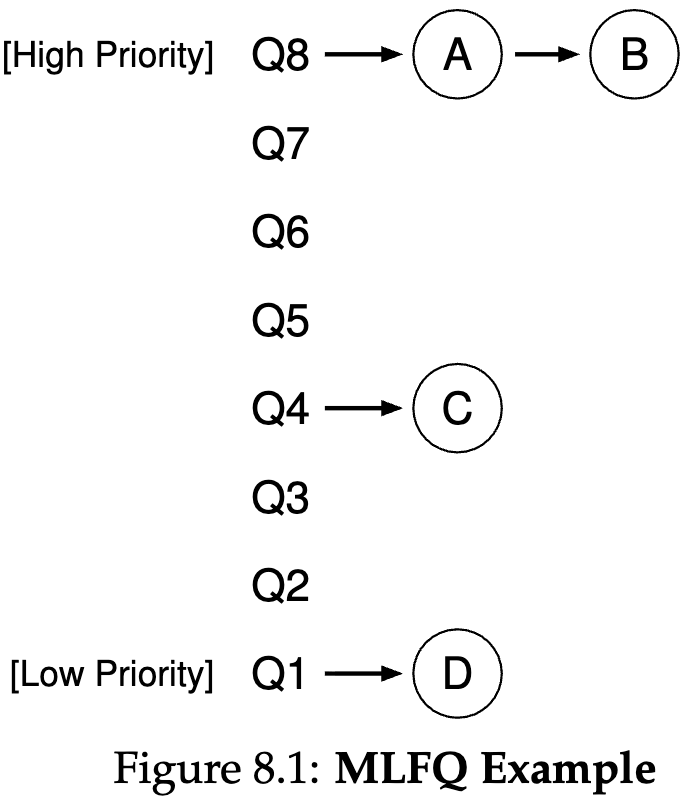
\includegraphics[width=1.1\linewidth]{figs/chapter-8/figure-8.1.png}
            \caption*{Source: chapter page 3.}
            \label{fig:figure-8.1}
        \end{figure}
    \end{columns}
\end{frame}

%------------------------------------------------

\begin{frame}{Changing Priority: First Attempt}
    \begin{itemize}
        \item A job's \textbf{allotment} is the amount of CPU time it may use
        at a priority level before being demoted.
        \item Initially, assume the allotment equals one time slice.
    \end{itemize}

    \begin{block}{Initial Priority Rules}
        \textbf{Rule 3:} A new job enters at the highest priority.\\[0.4em]

        \textbf{Rule 4a:} If a job uses its entire allotment, its priority is reduced.\\[0.4em]

        \textbf{Rule 4b:} If a job gives up the CPU before its allotment expires,
        it stays at the same priority.
    \end{block}
\end{frame}

%------------------------------------------------

\begin{frame}{Example 1: A Long-Running Job}
    \begin{columns}
        \column{0.48\textwidth}
        \begin{itemize}
            \item Consider three priority queues.
            \item Time slice: 10 ms.
            \item The job starts in the highest-priority queue.
            \item After consuming each allotment, it moves down one queue.
            \item Eventually, it remains in the lowest-priority queue.
        \end{itemize}

        \column{0.52\textwidth}
        \begin{figure}
            \centering
            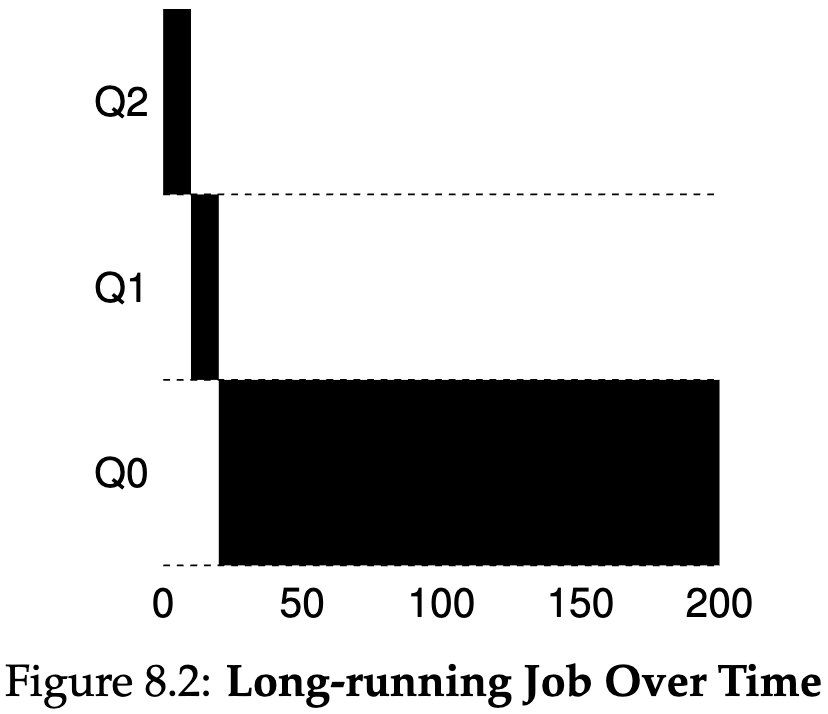
\includegraphics[width=1.1\linewidth]{figs/chapter-8/figure-8.2.png}
            \caption*{Source: chapter page 4.}
            \label{fig:figure-8.2}
        \end{figure}
    \end{columns}
\end{frame}

%------------------------------------------------

\begin{frame}{Example 2: A Short Job Arrives}
    \begin{columns}
        \column{0.48\textwidth}
        \begin{itemize}
            \item Job A is a long-running CPU-intensive job.
            \item Job B is a newly-arrived short job.
            \item B enters at the highest priority.
            \item Because B is short, it completes before reaching the lowest queue.
            \item MLFQ therefore approximates SJF without knowing job lengths.
        \end{itemize}

        \column{0.52\textwidth}
        \begin{figure}
            \centering
            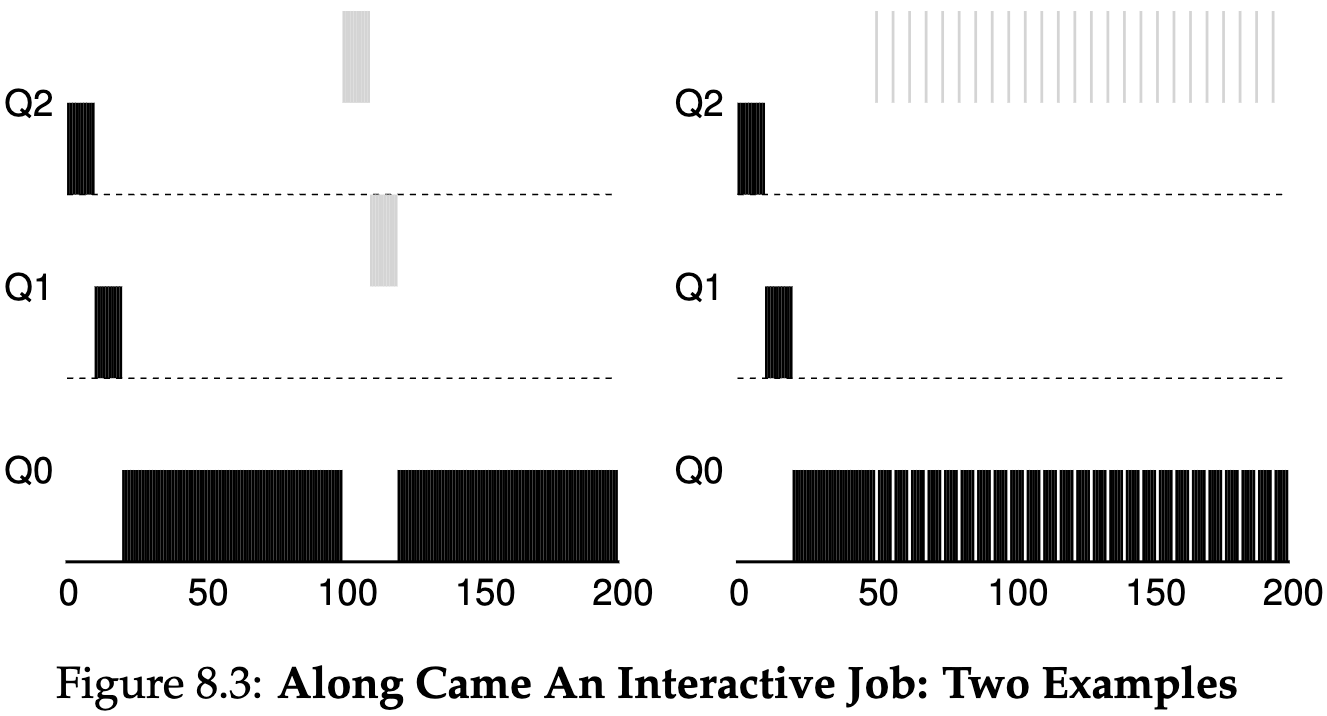
\includegraphics[width=1.1\linewidth]{figs/chapter-8/figure-8.3.png}
            \caption*{Source: chapter page 5.}
            \label{fig:figure-8.3-left}
        \end{figure}
    \end{columns}
\end{frame}

%------------------------------------------------

\begin{frame}{Example 3: Interactive Jobs and I/O}
    \begin{columns}
        \column{0.48\textwidth}
        \begin{itemize}
            \item Interactive jobs often relinquish the CPU for I/O.
            \item Under Rule 4b, such jobs remain at high priority.
            \item This allows interactive jobs to receive fast CPU service.
        \end{itemize}

        \column{0.52\textwidth}
        \begin{figure}
            \centering
            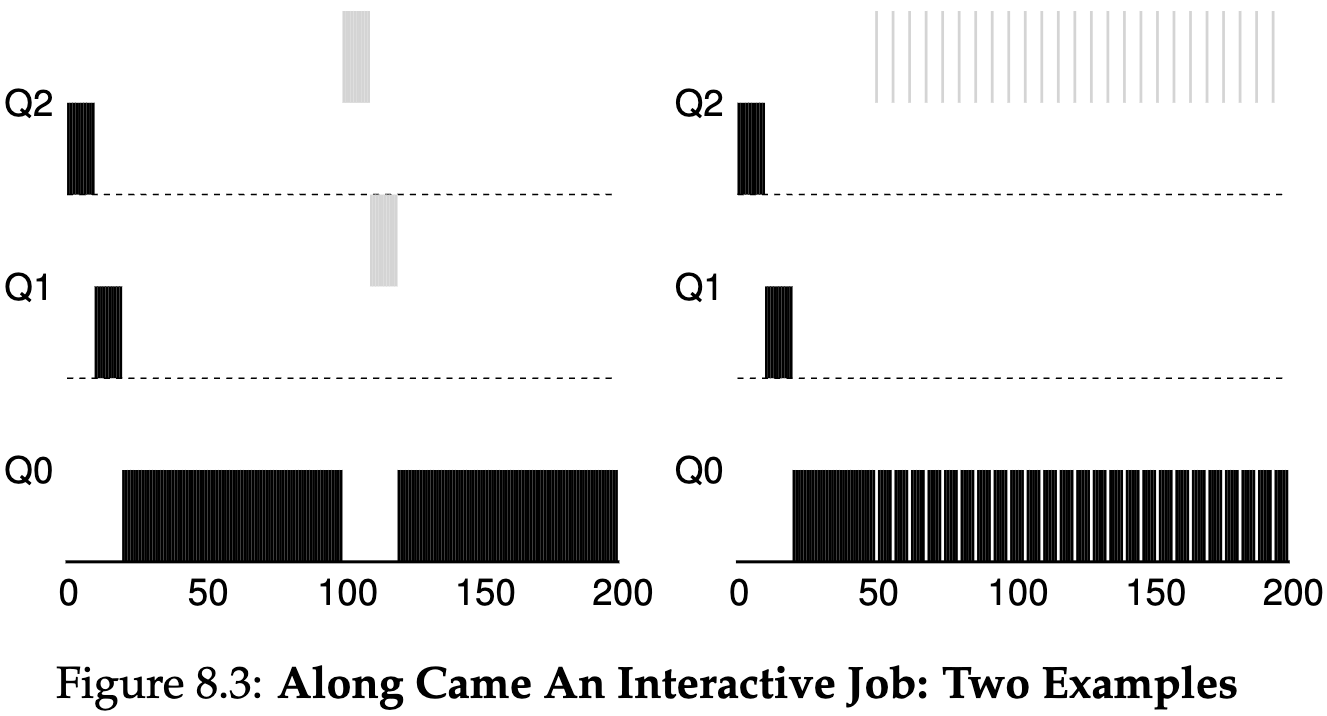
\includegraphics[width=1.1\linewidth]{figs/chapter-8/figure-8.3.png}
            \caption*{Source: chapter page 5.}
            \label{fig:figure-8.3-rigth}
        \end{figure}
    \end{columns}
\end{frame}

%------------------------------------------------

\begin{frame}{Problems With the Initial MLFQ}
    \begin{enumerate}
        \item \textbf{Starvation}
        \begin{itemize}
            \item Too many interactive jobs may consume all CPU time.
            \item Long-running jobs may never execute.
        \end{itemize}

        \item \textbf{Gaming the Scheduler}
        \begin{itemize}
            \item A job can issue I/O just before its allotment expires.
            \item It can remain at high priority and obtain an unfair CPU share.
        \end{itemize}

        \item \textbf{Changing Behavior}
        \begin{itemize}
            \item A CPU-bound process may later become interactive.
            \item The current rules do not adapt well to this change.
        \end{itemize}
    \end{enumerate}
\end{frame}

%------------------------------------------------

\begin{frame}{Attempt \#2: Priority Boost}
    \begin{block}{Rule 5}
        After some time period $S$, move all jobs in the system
        to the topmost queue.
    \end{block}

    \begin{itemize}
        \item Prevents starvation of long-running jobs.
        \item Allows jobs whose behavior changed to regain high priority.
        \item However, choosing a proper value for $S$ is difficult.
    \end{itemize}
\end{frame}

%------------------------------------------------

\begin{frame}{Priority Boost in Action}
    \begin{columns}
        \column{0.45\textwidth}
        \begin{itemize}
            \item Without priority boosts:
            \begin{itemize}
                \item a long-running job may starve.
            \end{itemize}

            \item With periodic boosts:
            \begin{itemize}
                \item the long-running job periodically receives CPU time.
            \end{itemize}
        \end{itemize}

        \column{0.55\textwidth}
        \begin{figure}
            \centering
            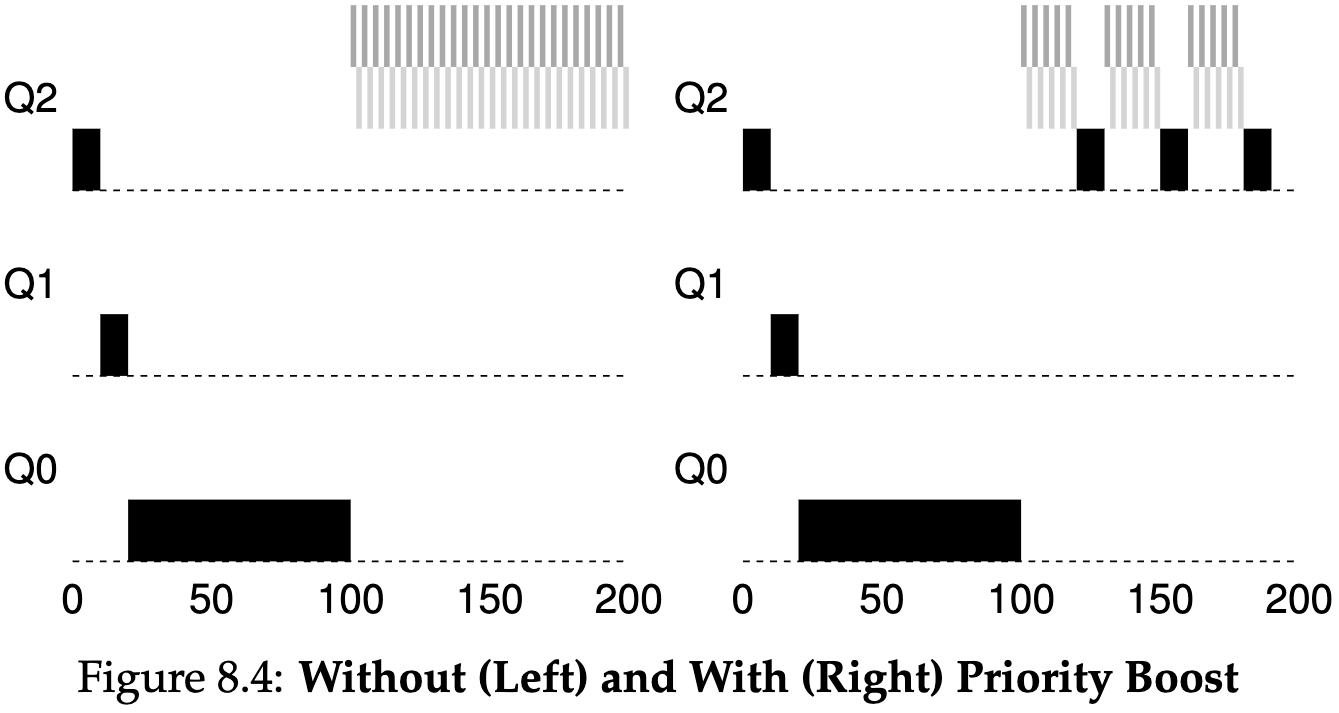
\includegraphics[width=1.1\linewidth]{figs/chapter-8/figure-8.4.png}
            \caption*{Source: chapter page 7.}
            \label{fig:figure-8.4}
        \end{figure}
    \end{columns}
\end{frame}

%------------------------------------------------

\begin{frame}{Attempt \#3: Better Accounting}
    \begin{itemize}
        \item Rules 4a and 4b allow processes to game the scheduler.
        \item The solution is to track the \textbf{total CPU time used at each level}.
        \item Giving up the CPU for I/O no longer resets the allotment.
    \end{itemize}

    \begin{block}{Revised Rule 4}
        Once a job uses up its time allotment at a given level,
        regardless of how many times it has given up the CPU,
        its priority is reduced.
    \end{block}
\end{frame}

%------------------------------------------------

\begin{frame}{Preventing Scheduler Gaming}
    \begin{columns}
        \column{0.45\textwidth}
        \begin{itemize}
            \item Old rules:
            \begin{itemize}
                \item I/O could be used to remain at high priority.
            \end{itemize}

            \item Better accounting:
            \begin{itemize}
                \item CPU usage is accumulated.
                \item The process eventually moves down the queues.
            \end{itemize}
        \end{itemize}

        \column{0.55\textwidth}
        \begin{figure}
            \centering
            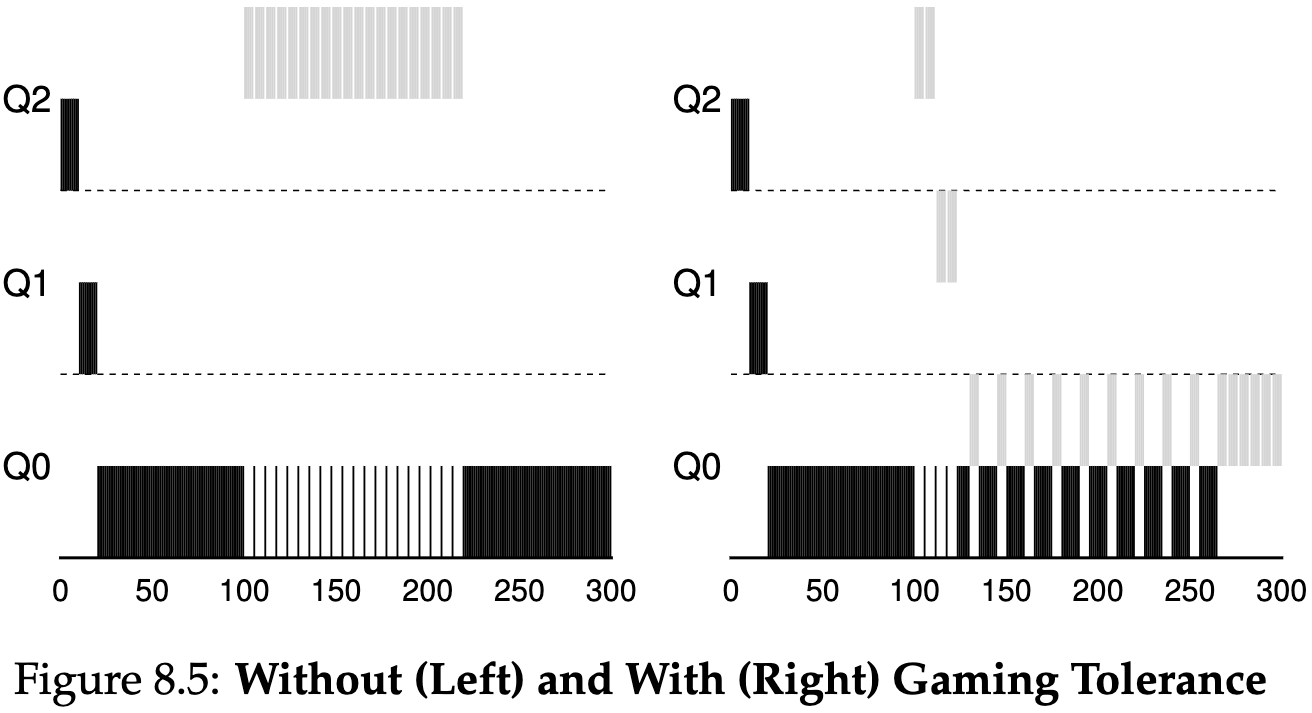
\includegraphics[width=1.1\linewidth]{figs/chapter-8/figure-8.5.png}
            \caption*{Source: chapter page 8.}
            \label{fig:figure-8.5}
        \end{figure}
    \end{columns}
\end{frame}

%------------------------------------------------

\begin{frame}{Tuning MLFQ}
    \begin{itemize}
        \item Important parameters include:
        \begin{itemize}
            \item number of queues;
            \item time slice per queue;
            \item allotment per priority level;
            \item frequency of priority boosts.
        \end{itemize}

        \item High-priority queues usually use \textbf{short time slices}.
        \item Low-priority queues usually use \textbf{longer time slices}.
        \item Interactive jobs benefit from quick switching.
        \item CPU-bound jobs benefit from longer uninterrupted execution.
    \end{itemize}
\end{frame}

%------------------------------------------------

\begin{frame}{Lower Priority, Longer Quanta}
    \begin{columns}
        \column{0.45\textwidth}
        \begin{itemize}
            \item Example:
            \begin{itemize}
                \item highest queue: 10-ms time slice;
                \item middle queue: 20-ms time slice;
                \item lowest queue: 40-ms time slice.
            \end{itemize}
        \end{itemize}

        \column{0.55\textwidth}
        \begin{figure}
            \centering
            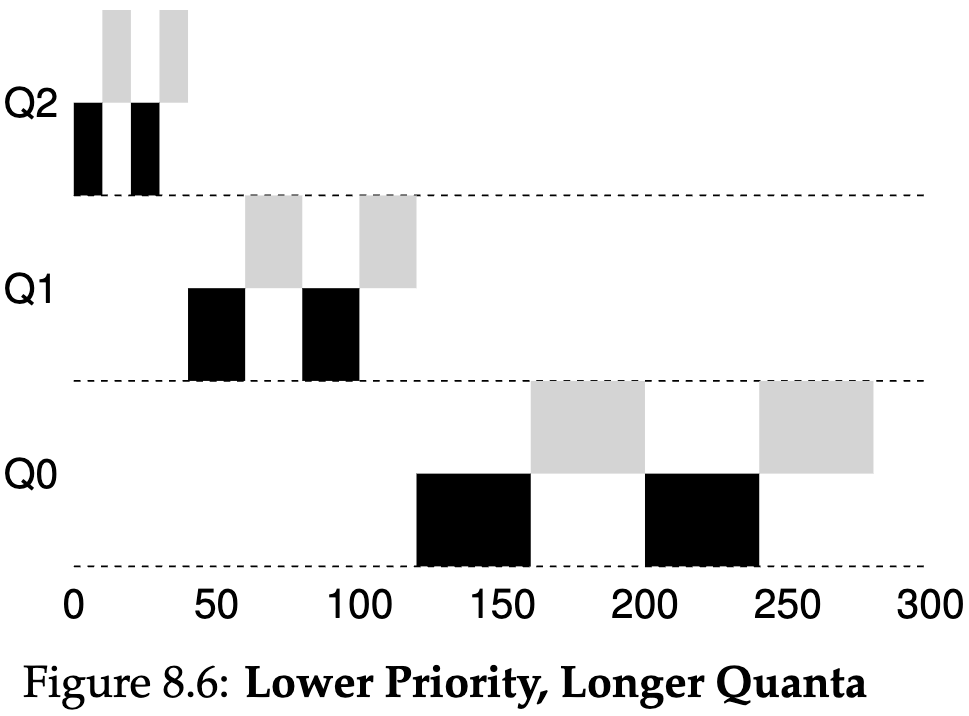
\includegraphics[width=1.1\linewidth]{figs/chapter-8/figure-8.6.png}
            \caption*{Source: chapter page 9.}
            \label{fig:figure-8.6}
        \end{figure}
    \end{columns}
\end{frame}

%------------------------------------------------

\begin{frame}{MLFQ in Real Systems}
    \begin{itemize}
        \item Different systems implement variations of MLFQ.
        \item Solaris Time-Sharing (TS):
        \begin{itemize}
            \item configurable priority tables;
            \item 60 queues in the default configuration;
            \item increasing time-slice lengths at lower priorities;
            \item periodic priority boosts.
        \end{itemize}

        \item FreeBSD uses mathematical formulas based on CPU usage.
        \item Some systems reserve the highest priority levels for OS work.
        \item Utilities such as \texttt{nice} allow users to provide scheduling advice.
    \end{itemize}
\end{frame}

%------------------------------------------------

\begin{frame}{MLFQ: Final Rules}
    \small
    \begin{enumerate}
        \item If Priority(A) $>$ Priority(B), A runs.
        \item If Priority(A) = Priority(B), A and B run in Round Robin.
        \item New jobs enter the system at the highest priority.
        \item Once a job uses its time allotment at a level, its priority is reduced.
        \item After some period $S$, all jobs are moved to the highest-priority queue.
    \end{enumerate}
\end{frame}

%------------------------------------------------

\begin{frame}{Summary}
    \begin{itemize}
        \item MLFQ uses multiple priority queues and feedback from job behavior.
        \item It does not require a priori knowledge of job length.
        \item Short and interactive jobs tend to remain at high priority.
        \item CPU-intensive jobs gradually move to lower-priority queues.
        \item Priority boosts prevent starvation and adapt to behavioral changes.
        \item Better accounting prevents jobs from gaming the scheduler.
        \item MLFQ combines good responsiveness with progress for long-running jobs.
    \end{itemize}
\end{frame}

%------------------------------------------------